\chapter{数据集构建与 Bug 修复识别}\label{chap:dataset}

\section{数据概览与初步量化分析}

本研究的数据来自仓库中已整理的提交级 CSV 文件与汇总报告。为了从宏观角度审视 PostgreSQL（2022--2025）的维护情况，我们首先对整体提交规模进行统计。

\begin{figure}[htbp]
    \centering
    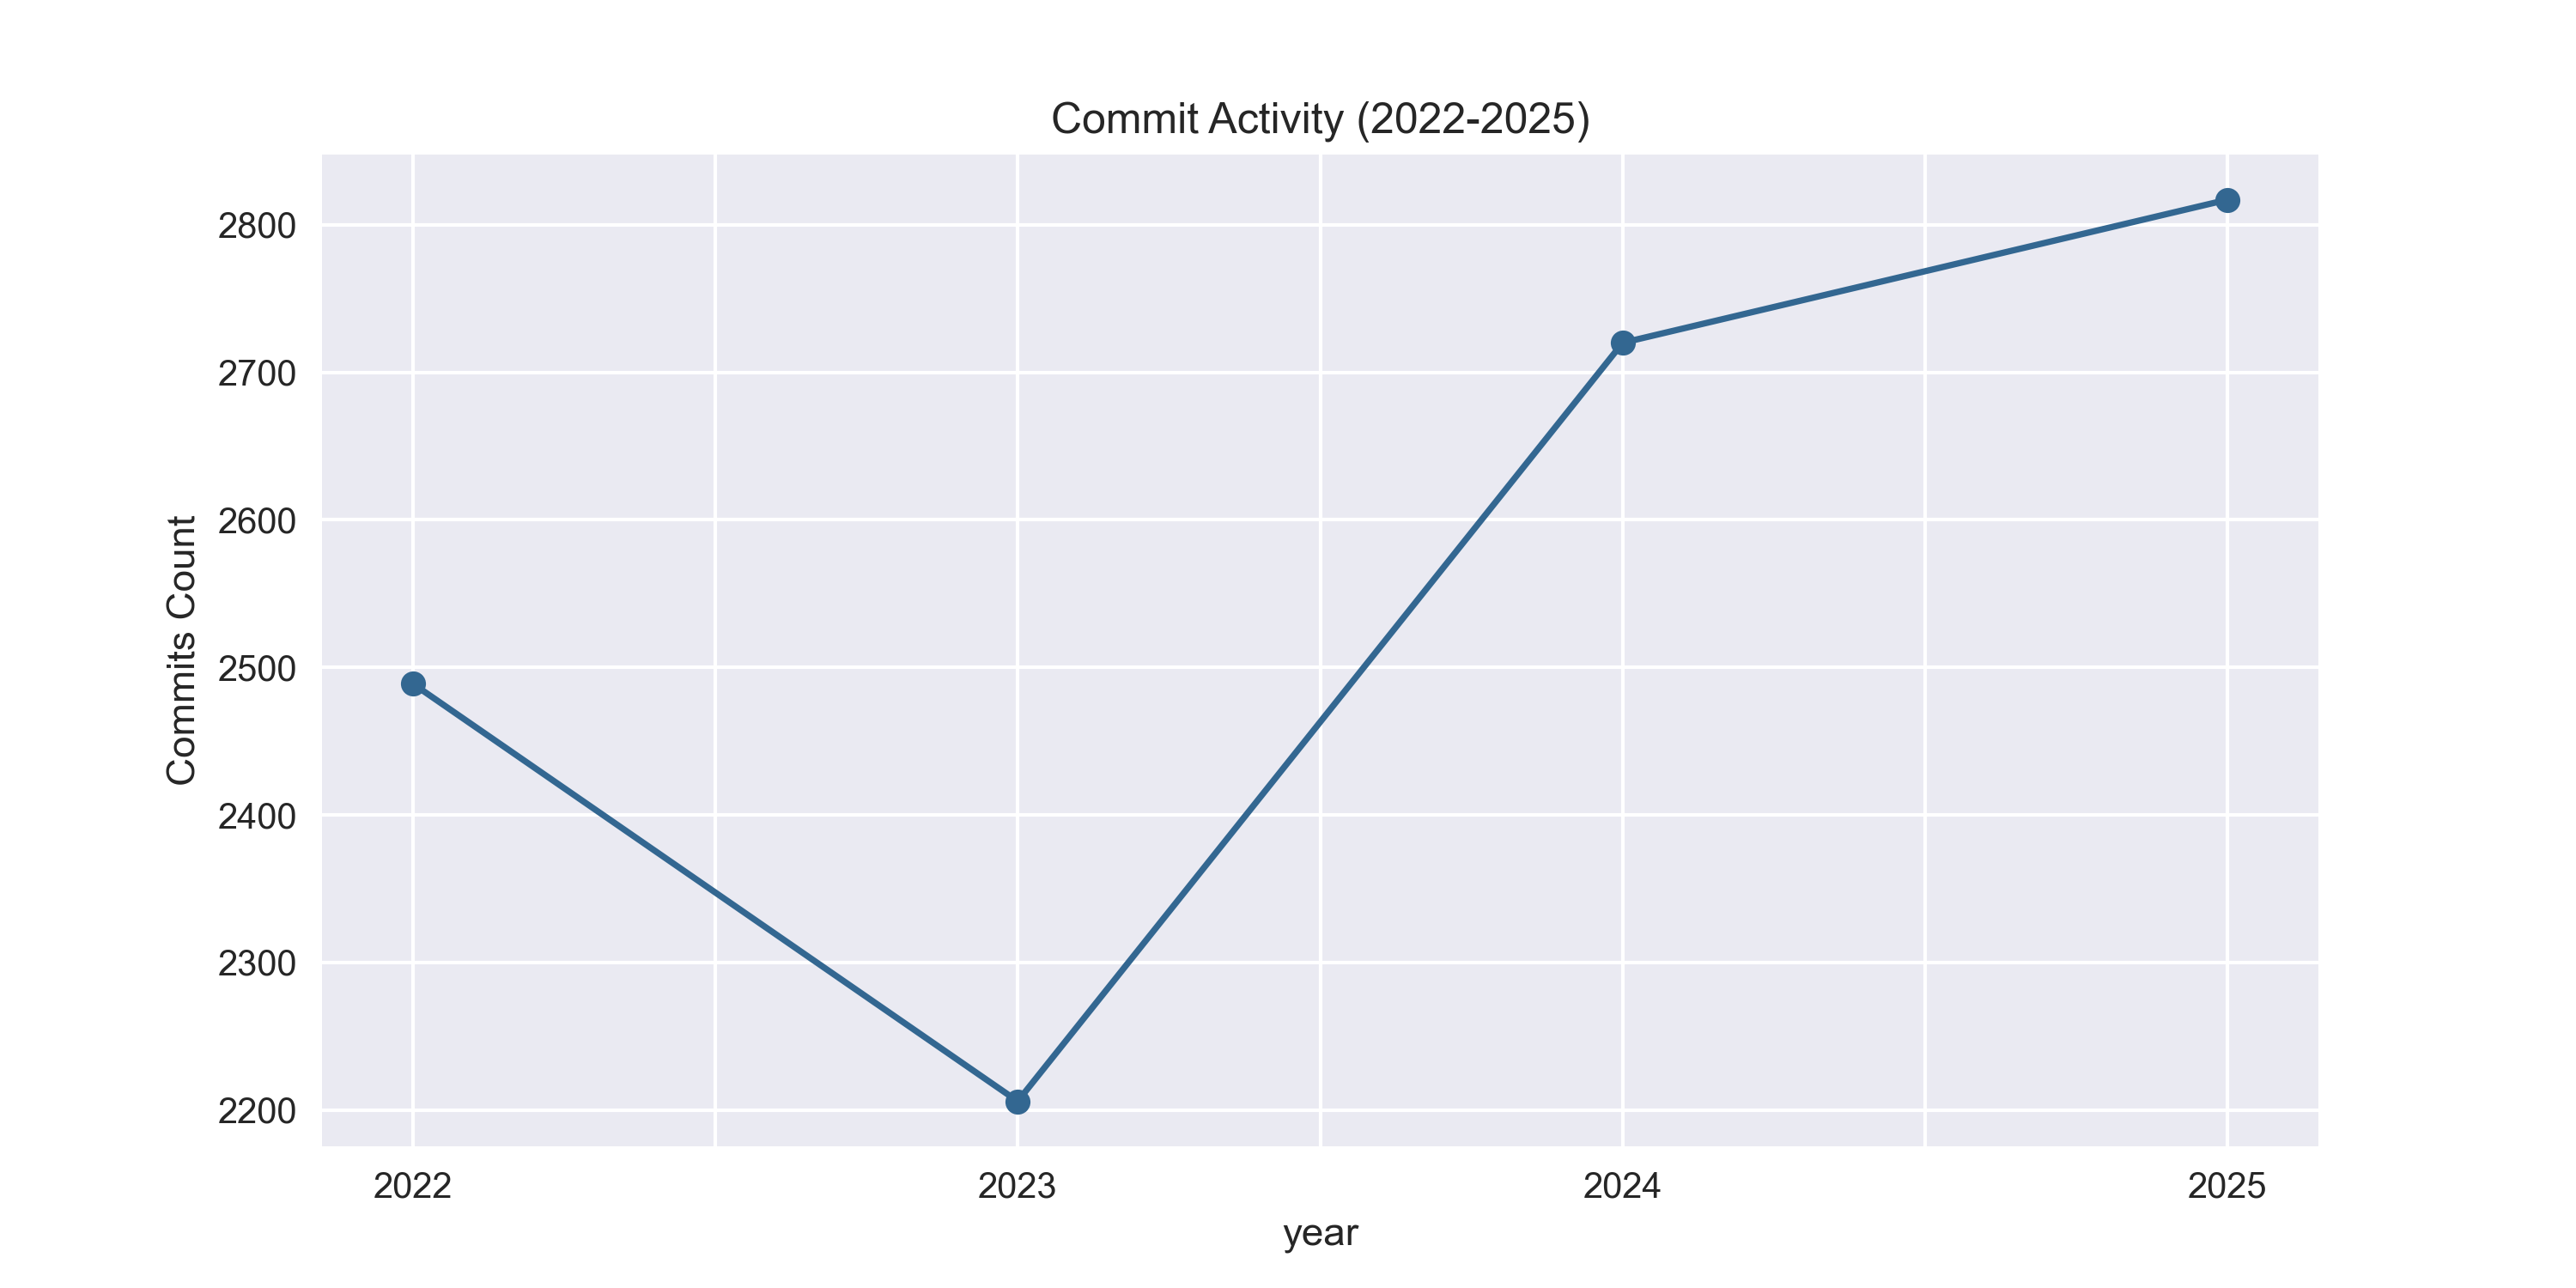
\includegraphics[width=0.85\textwidth]{Img/commit_trend.png} 
    \caption{2022--2025年 PostgreSQL 修复提交数量年度分布图}
    \label{fig:annual_stats}
\end{figure}



依据图 \ref{fig:annual_stats} 所示，2022--2025 年的修复提交数量分别为 692、619、820、829，四年合计 2960 次。数据显示，2024 年和 2025 年的修复活跃度较往年有显著提升，这为本研究提供了充足且高质量的分析样本。

\section{Bug 修复识别规则与标注流程}

\subsection{识别规则}
本研究采用三类信号联合识别策略：
\begin{itemize}
    \item \textbf{关键词信号}：优先捕获 \texttt{fix, crash, leak, assert} 等强语义词汇；
    \item \textbf{结构信号}：监测代码中是否出现条件检查新增、错误处理 API 强化；
    \item \textbf{测试信号}：检查 \texttt{src/test} 目录下是否存在同步的回归测试更新。
\end{itemize}

\subsection{标注流程与质量控制}
标注流程遵循“规则筛查 + 人工复核”两阶段。通过 \texttt{git log --grep} 生成候选集后，对候选逐条执行 \texttt{git show -U3}，按 \textbf{Y/M/N}（明确修复/疑似/非修复）标注。针对 \texttt{storage} 等高风险模块执行二人复核，保留冲突裁决记录。

\section{描述性统计分析}

本节针对标注后的数据集，从复杂度、贡献度及模块分布三个维度进行详细分析。

\subsection{修复复杂度分析}

为了衡量修复的深度，我们对补丁的代码变更行数（Churn）与逻辑复杂度进行了挖掘。

\begin{figure}[htbp]
    \centering
    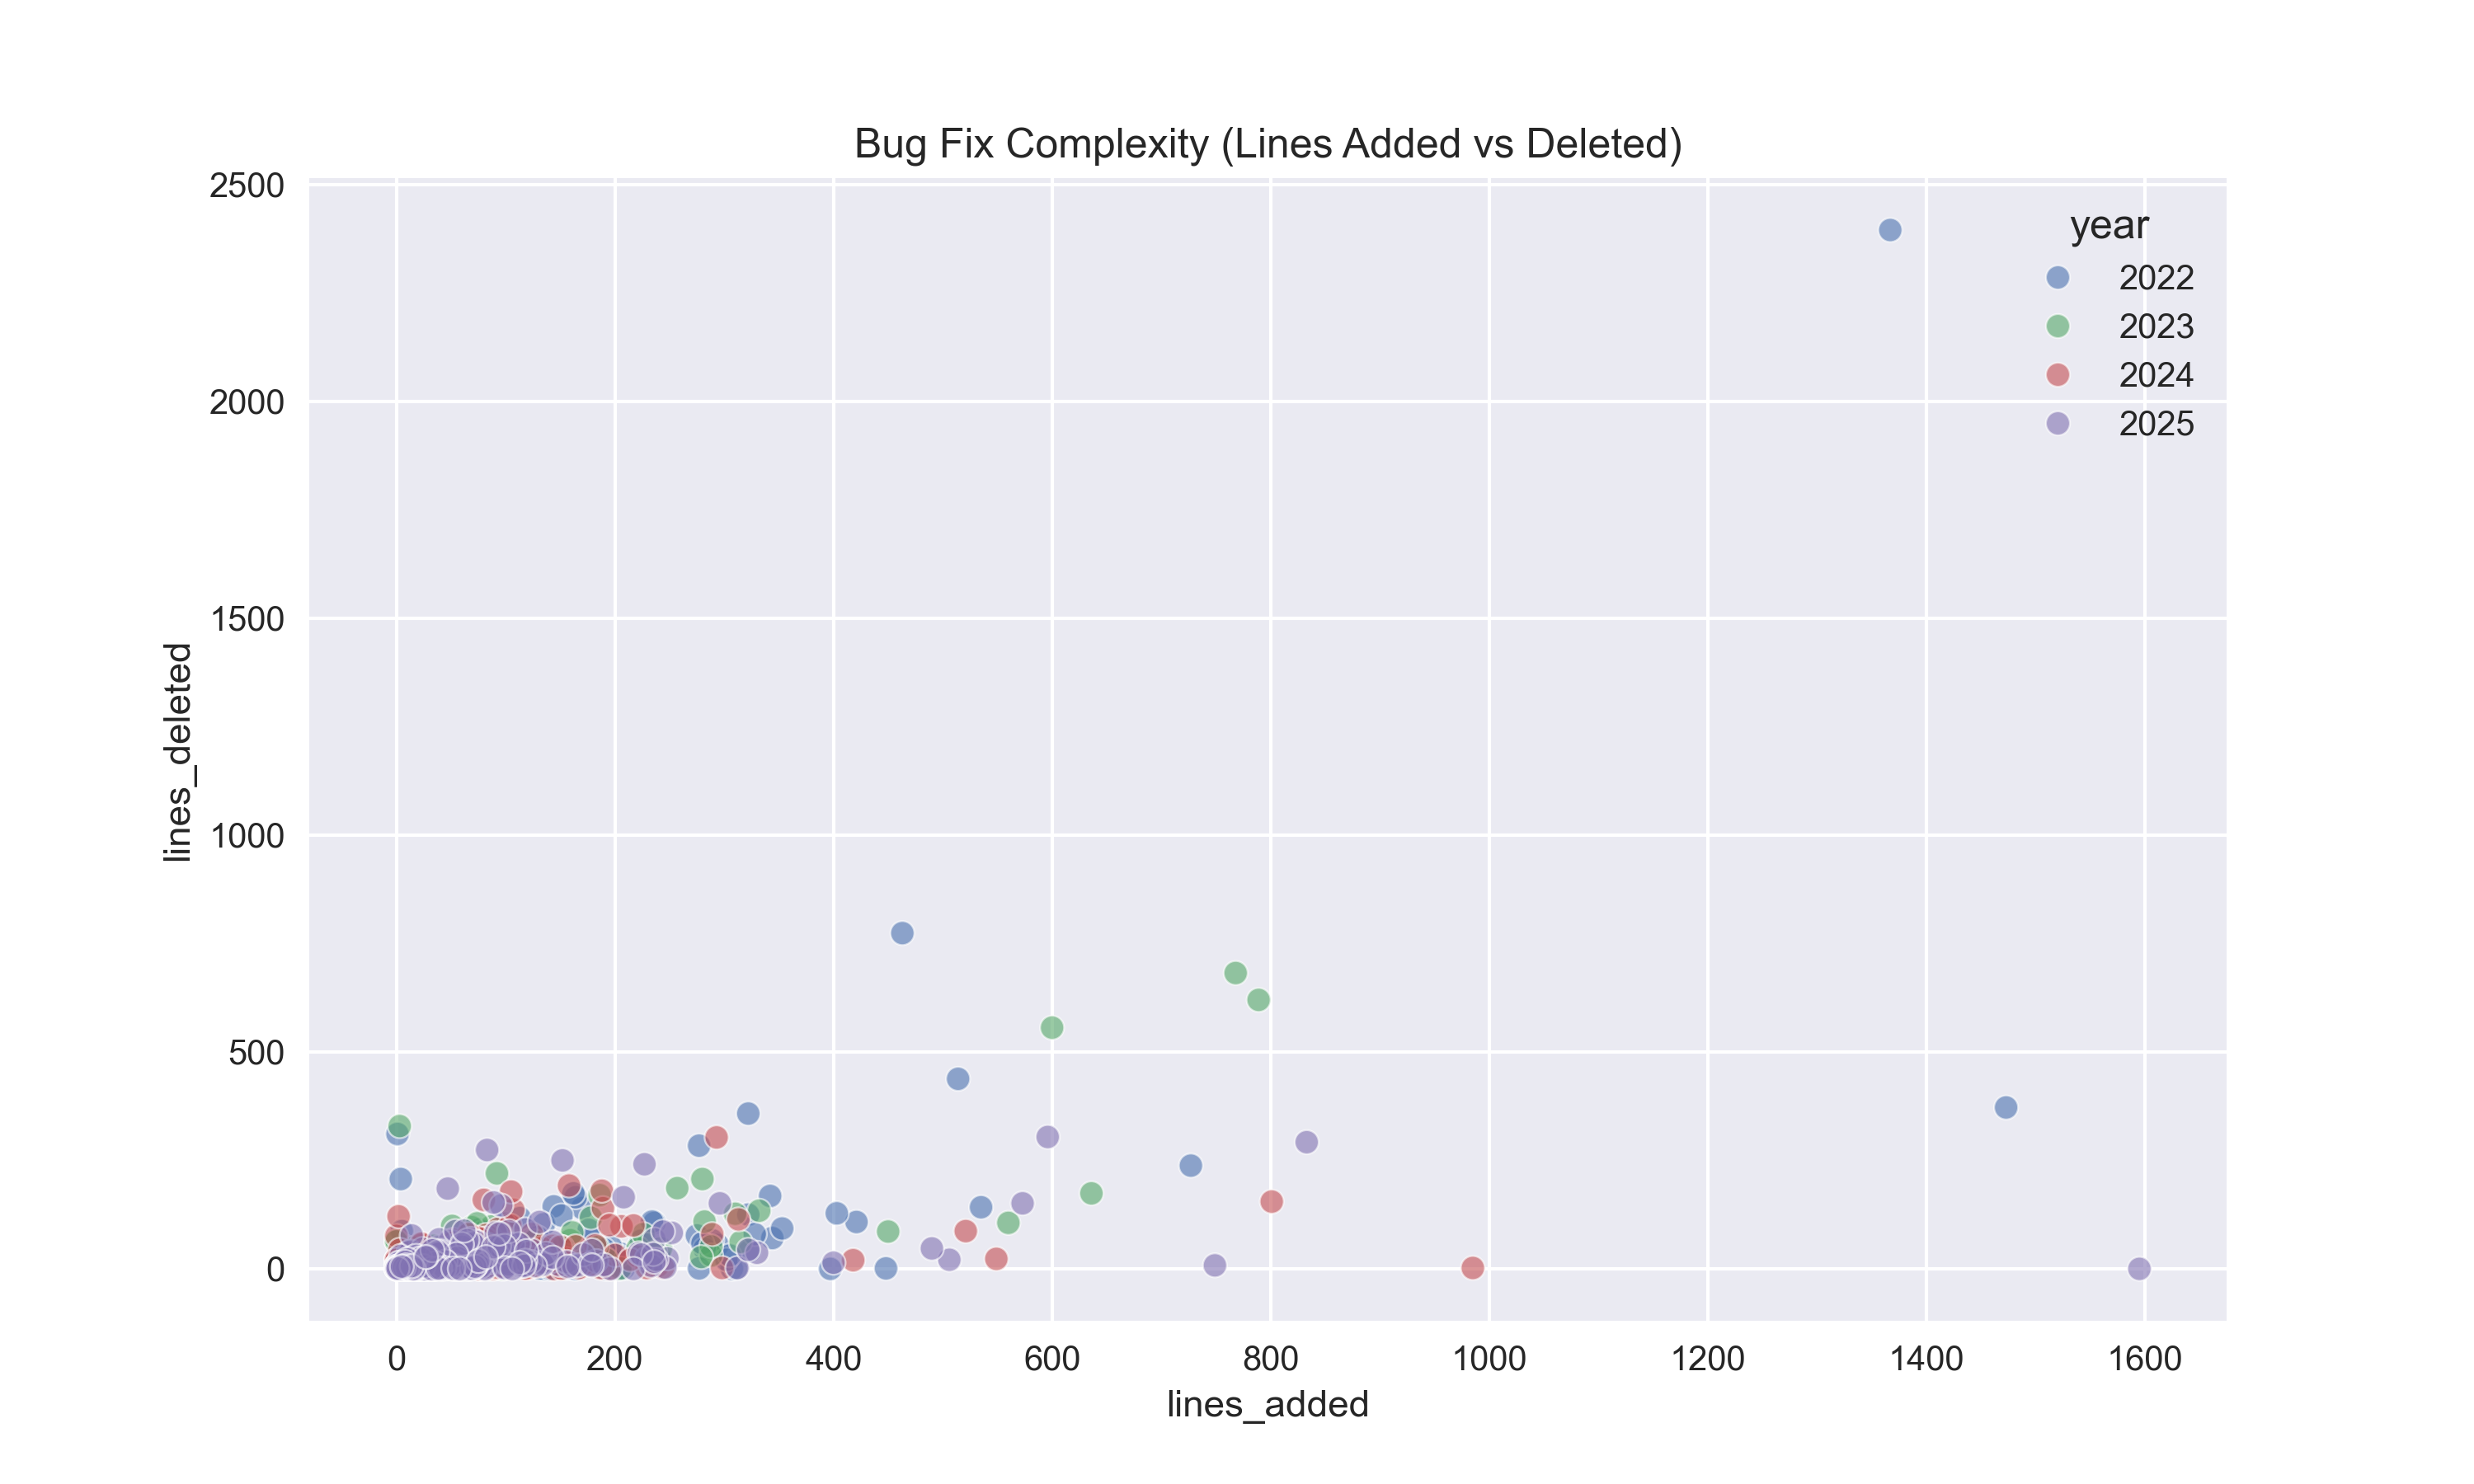
\includegraphics[width=0.85\textwidth]{Img/complexity_analysis.png} 
    \caption{Bug 修复补丁的增添复杂度分布分析}
    \label{fig:complexity}
\end{figure}



结合图 \ref{fig:complexity} 的数据，2022--2025 年对应年度 churn 分别为 41610、30477、34469、36852 行。中位新增/删除行为 7/3 行，新增行 P90 约为 79 行。这说明 PostgreSQL 的多数修复属于“小步快修”模式，旨在最小化对核心系统的冲击，但在逻辑密集模块仍存在复杂度极高的大规模补丁。

\subsection{作者贡献度分布}

通过分析提交元数据中的作者字段，我们可以识别出社区中承担修复工作的主要群体。

\begin{figure}[htbp]
    \centering
    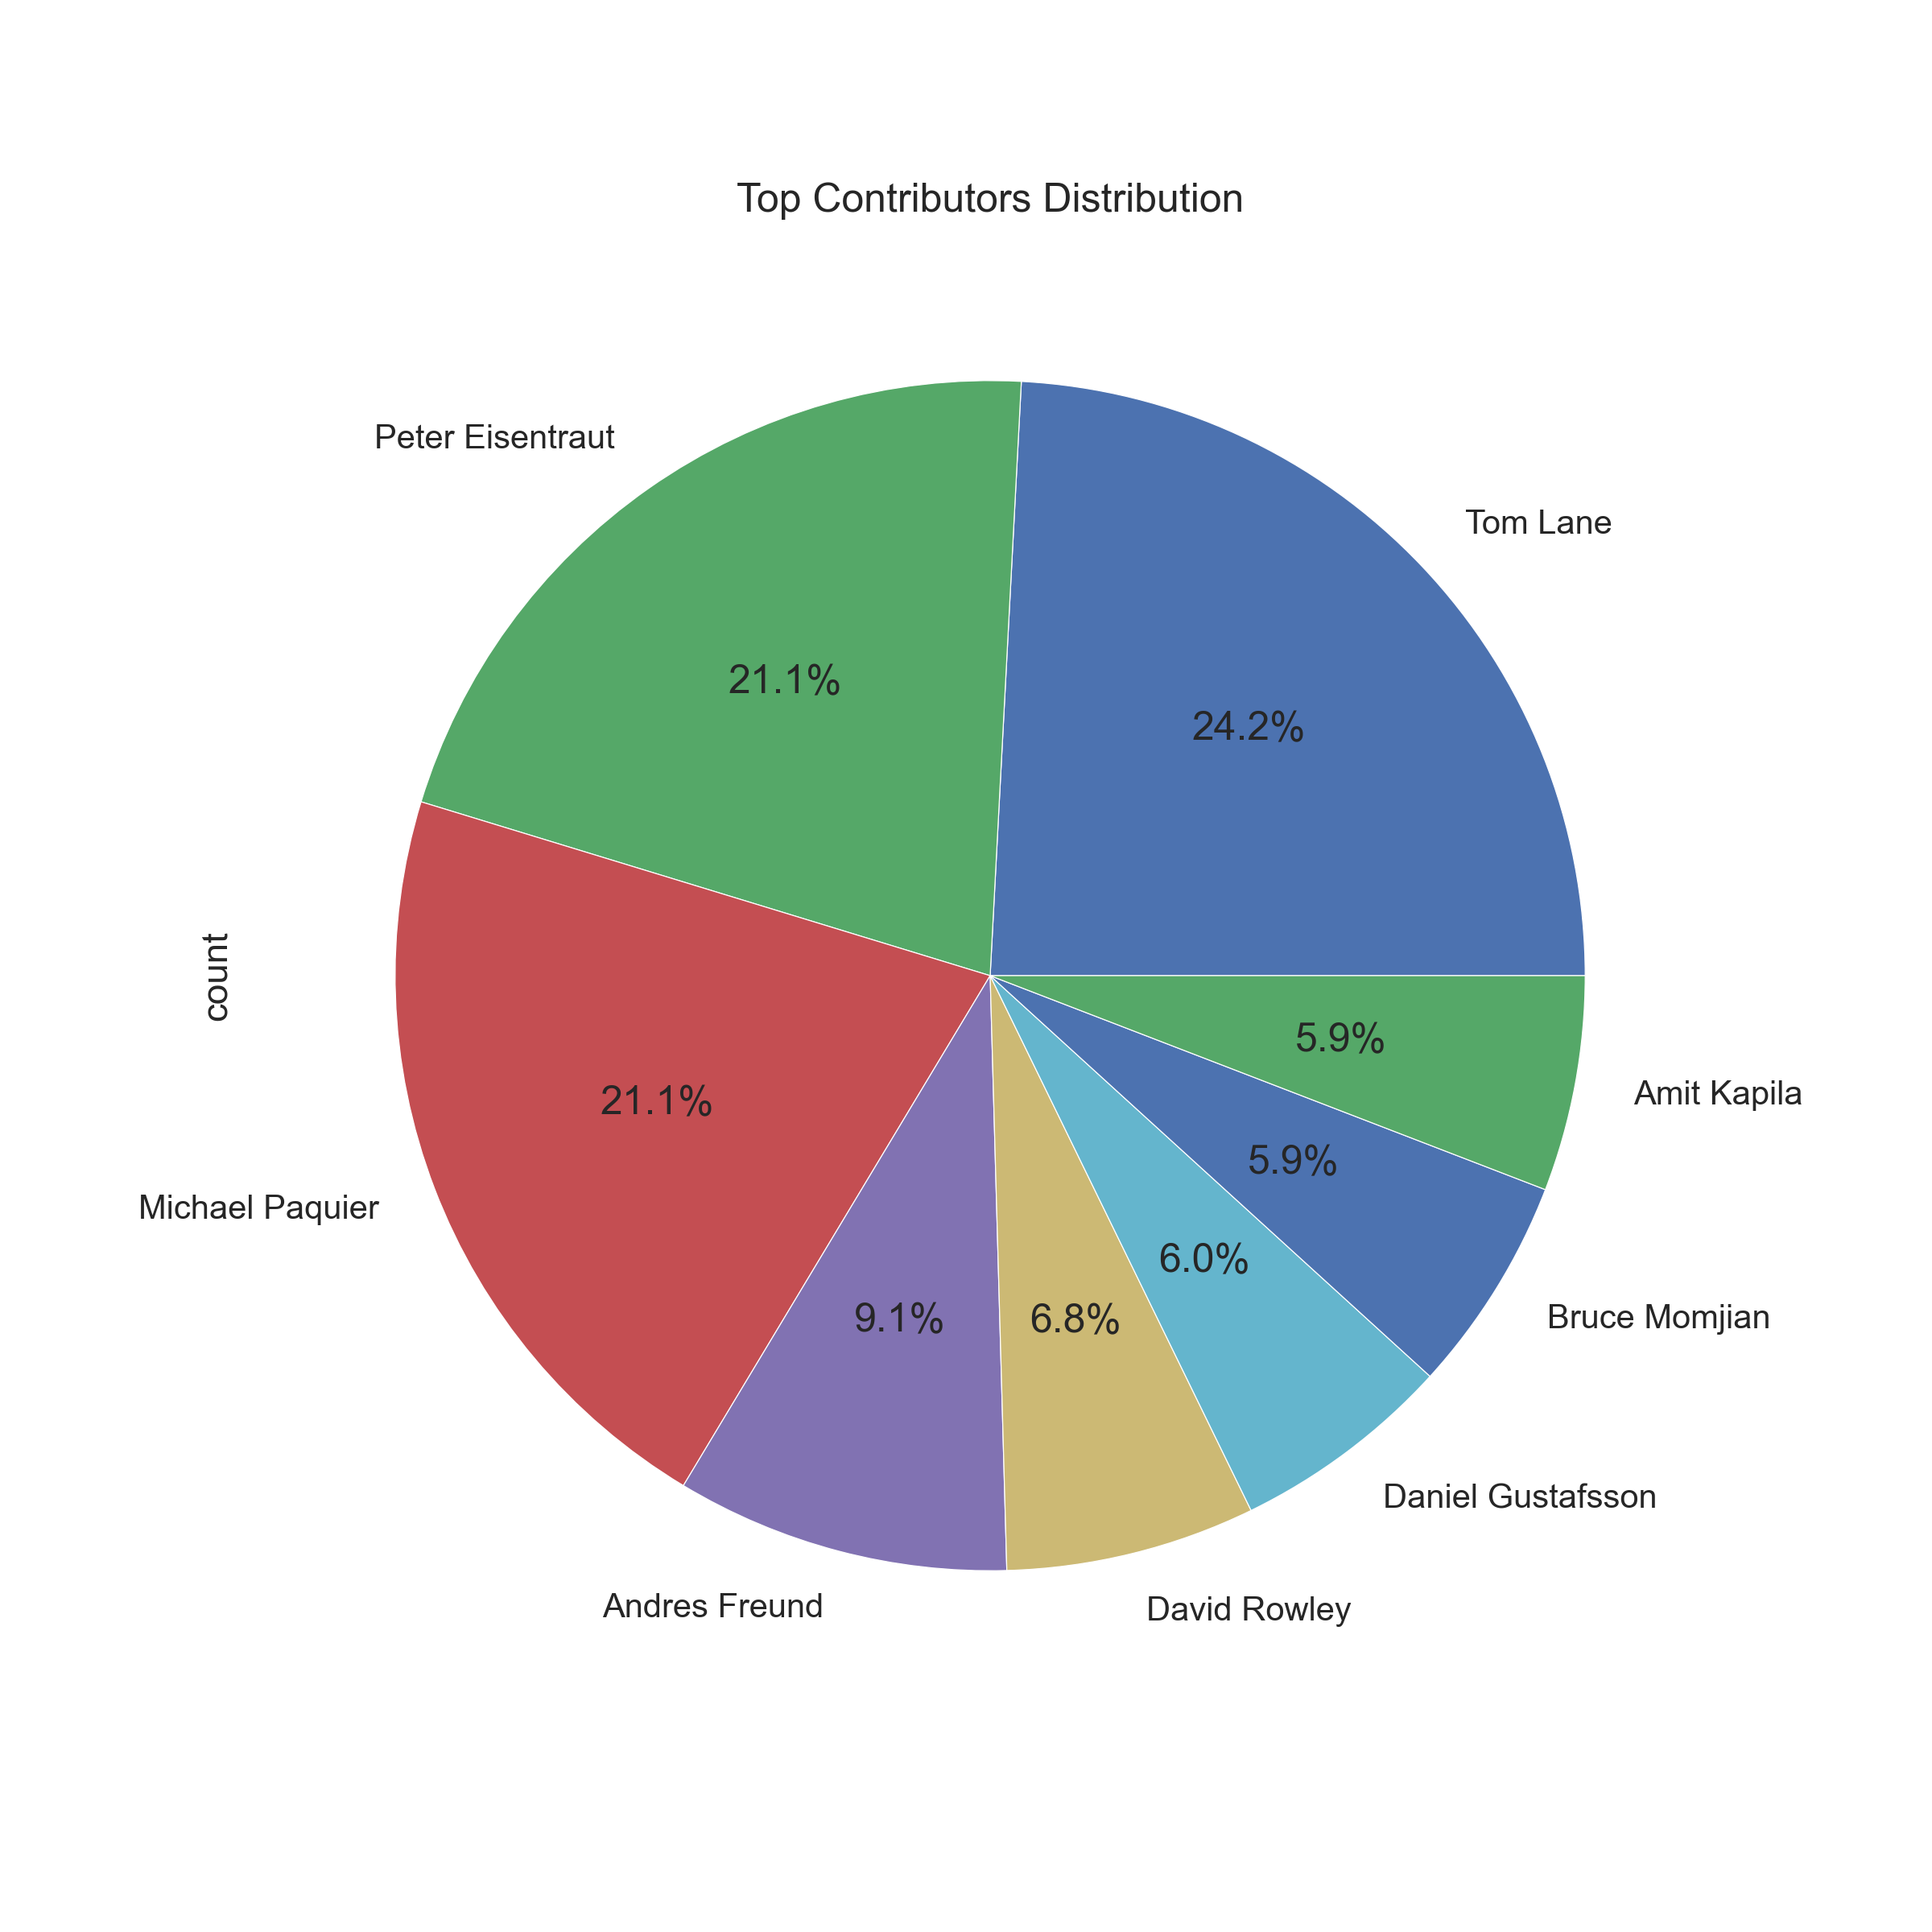
\includegraphics[width=0.75\textwidth]{Img/contributor_distribution.png} 
    \caption{PostgreSQL 核心贡献者修复提交占比统计}
    \label{fig:author_dist}
\end{figure}



如图 \ref{fig:author_dist} 所示，Top-3 作者分别为 Tom Lane（497 次）、Michael Paquier（463 次）和 Peter Eisentraut（309 次）。前三位作者的贡献量合计约占总体的 41.2\%。这一结果表明，PostgreSQL 的核心维护者在系统稳定性的保障中发挥了主导作用，其修复模式具有极高的研究价值。

\subsection{模块分布特征}
在 677 条静态分析样本中，路径聚合显示 \texttt{replication} 与 \texttt{storage} 各 45 条，\texttt{wal} 相关 13 条。验证了高风险底层模块长期承受着较高的修复压力，这也是后续章节进行形式化验证的重点关注领域。

本章得到的数据与标注结果，为后续章节的分析提供了统一样本基础。